\chapter{Les différents modes de fonctionnement de l'AES}
\label{chap:différents modes}

Il existe plusieurs modes de fonctionnenement de l'AES, comme l'\aes. Nous présenterons ici les plus utilisés.

\section{ECB}

Le mode ECB (Electronic codebook ou dictionnaire de code) est le plus simple. Il consiste à diviser le message à chiffrer en blocs qui vont être chiffrés indépendament les uns des autres. Pour le déchiffrement on procédera de la même manière en découpant le texte chiffré en blocs et en décryptant les blocs indépendament les uns des autres.

\begin{figure}[!h]
  \centering
  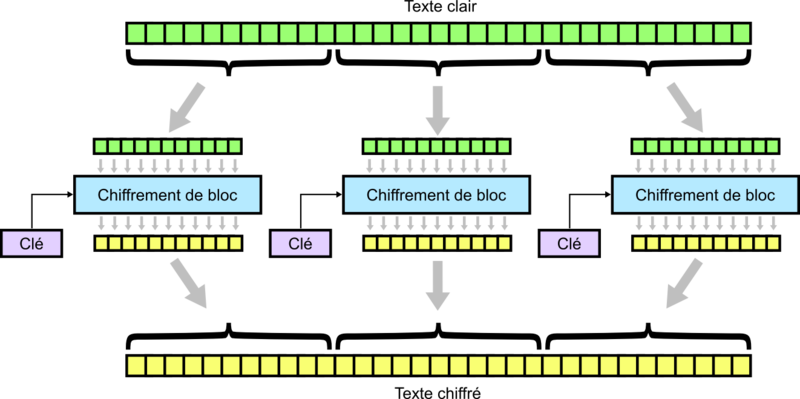
\includegraphics[width=\textwidth]{fonctionnement-ECB}
  \caption{schéma ECB \cite{wiki}}
  \label{schema ECB}
\end{figure}

Ce mode présente les avantages du chiffrement par flots, est pré-calculable et est parallélisable. Il offre la possibilité de déchiffrer une zone quelconque du texte chiffré et ainsi de déchiffrer une partie seulement des données.

Cependant ce mode possède un défaut considérable: deux blocs de texte clair seront chiffrés de la même manière, car il n'y a pas de randomisation. Ce défaut rend le mode ECB vulnérable aux attaques par dictionnaire et à l'analyse fréquentielle. En effet pour une clef donnée, on pourra générer un dictionnaire avec les correspondances entre les clairs et le chiffrés, permettant ainsi de retrouver le texte clair. Pour ces raisons l'utilisation de ce mode est fortement déconseillé.

\section{CBC}

Avec le mode CBC (Cipher Block Chainning ou Enchaînement des blocs), on applique à chaque bloc de texte clair un "XOR" (ou exclusif) avec le bloc chiffré précedent. Ainsi chaque bloc chiffré dépend des blocs traités auparavavant. Pour le premier bloc il faut fournir un vecteur d'initialisation.

\begin{figure}[!h]
  \centering
  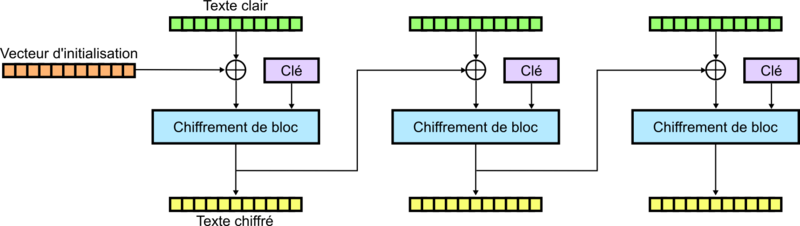
\includegraphics[width=\textwidth]{fonctionnement-CBC}
  \caption{schema CBC - Chiffrement \cite{wiki}}
  \label{schema CBC - Chiffrement}
\end{figure}

Ce mode présente possède les avantages du chiffrement par flots, et il offre également la possibilité de déchiffrer une zone quelconque du texte chiffré. Cependant un des inconvénients est que le chiffrement est séquentiel ( \cad il ne peut pas être parallélisé).

Pour le déchiffrement, on passe le premier bloc crypté dans le déchiffrement de bloc et on effectue un "XOR" avec le vecteur d'initialisation IV. Dans le cas où le vecteur d'initialisation est incorrect seul le premier bloc crypté sera impossible à décrypter. En effet à chaque bloc on applique un "XOR" avec le chiffré du bloc précédent, et pas le texte clair. Ainsi on peut retrouver un bloc de texte clair uniquement à partir du bloc crypté précédent, ce qui permet ainsi la parallélisation de la décryption. 

\begin{figure}[!h]
  \centering
  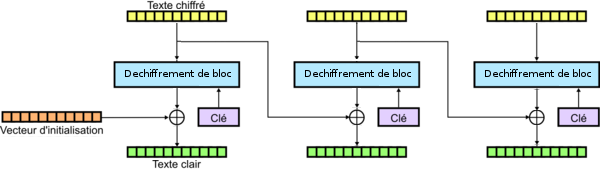
\includegraphics[width=\textwidth]{fonctionnement-CBC_de}
  \caption{schema CBC - Déchiffrement}
  \label{schema CBC - Déchiffrement}
\end{figure}




\section{CFB}
Le mode CFB (Cipher FeedBack ou Chiffrement à rétroaction) est similaire au mode CBC. Tout comme le CBC, ce mode permet de déchiffrer n'importe quelle zone du chiffré. Cependant, comme le CBC, le chiffrement est séquentiel, il ne peut donc pas être parallèlisé. Le déchiffrement est similaire au CBC et peut, quant à lui, être parallélisé. 

\begin{figure}[!h]
  \centering
  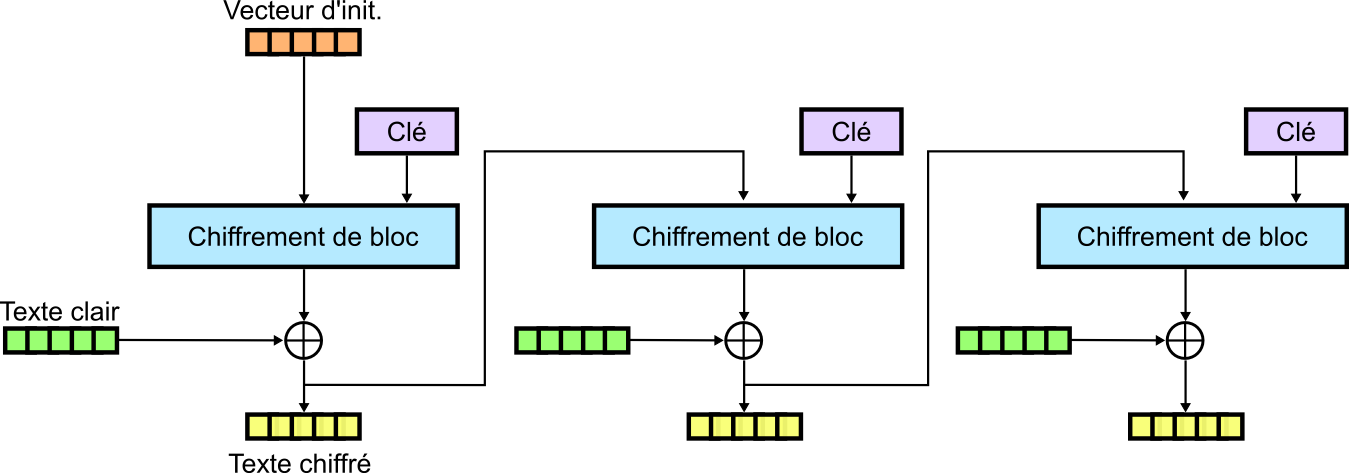
\includegraphics[width=\textwidth]{fonctionnement-CFB}
  \caption{schema CFB - Chiffrement}
  \label{schema CFB - Chiffrement}
\end{figure}

\begin{figure}[!h]
  \centering
  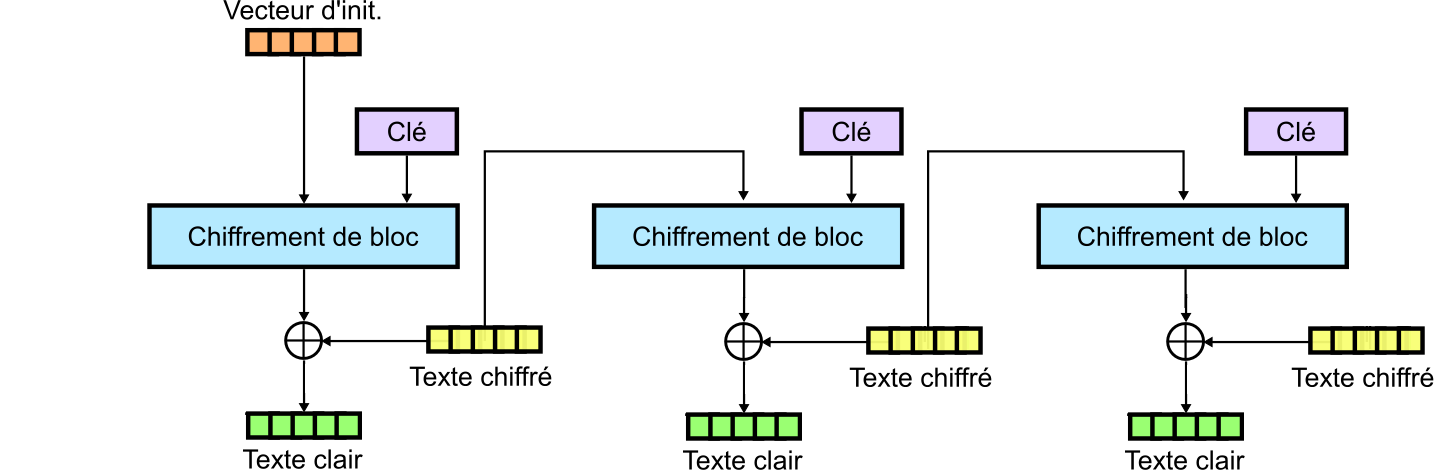
\includegraphics[width=\textwidth]{fonctionnement-CFB_de}
  \caption{schema CFB - Déchiffrement}
  \label{schema CFB - Déchiffrement}
\end{figure}

\section{OFB}
Le mode OFB (Output FeedBack) est une variante du mode CFB. En effet, au lieu d'utiliser un bloc chiffré pour chiffrer le suivant, le mode OFB va utiliser le chiffré du vecteur d'initialisation. S'il s'agit du bloc N, alors celui-ci sera chiffré avec le vecteur d'initialisation chiffré N fois. Le décryptage est très proche du CFB, il faut juste prendre le déchiffré du vecteur d'initialisation.


\begin{figure}[!h]
  \centering
  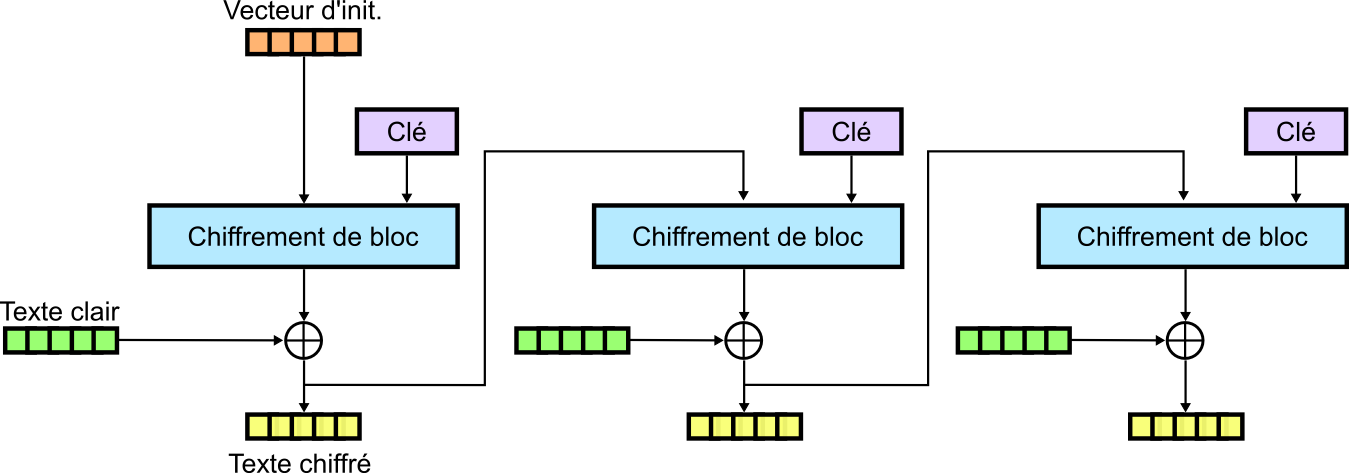
\includegraphics[width=\textwidth]{fonctionnement-OFB}
  \caption{schema OFB - Chiffrement}
  \label{schema OFB - Chiffrement}
\end{figure}

\begin{figure}[!h]
  \centering
  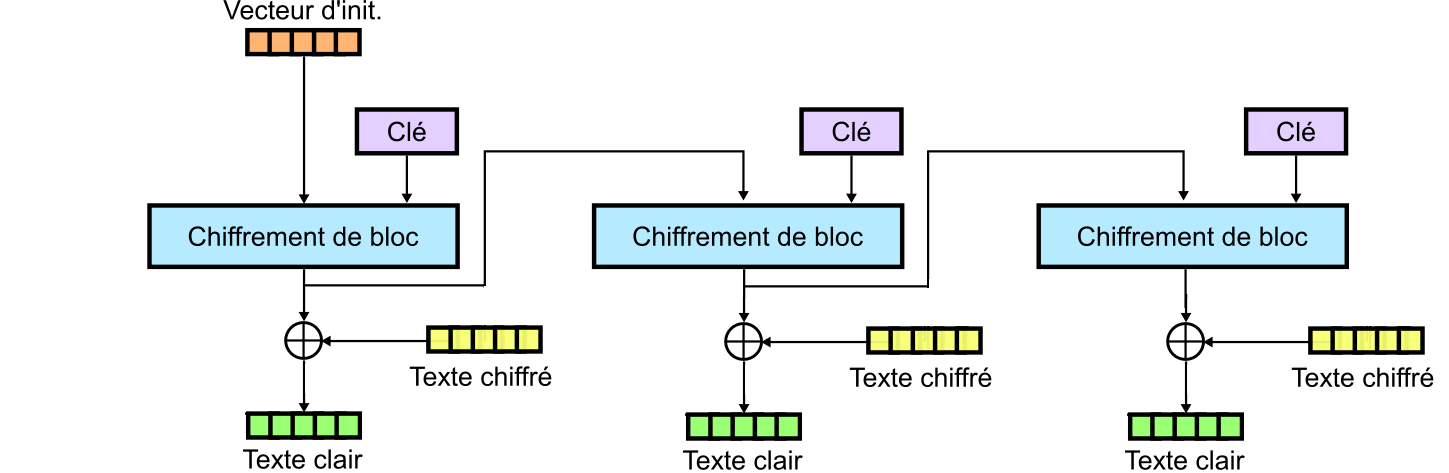
\includegraphics[width=\textwidth]{fonctionnement-OFB_de}
  \caption{schema OFB - Déhiffrement}
  \label{schema OFB - Déchiffrement}
\end{figure}

\section{CTR}
Comme le mode OFB, le mode CTR permet le chiffrement par flot et est pré-calculable. De plus il offre un accès aléatoire aux données, est parallélisable et n'utilise que la fonction de chiffrement. 

\begin{figure}[!h]
  \centering
  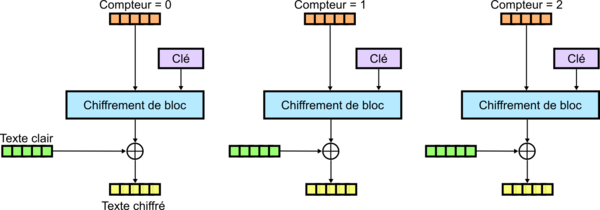
\includegraphics[width=\textwidth]{fonctionnement-CTR}
  \caption{schema CTR - Chiffrement}
  \label{schema CTR - Chiffrement}
\end{figure}


%%% Local Variables: 
%%% mode: latex
%%% TeX-master: "rapport_de_base"
%%% End: 
